

% A Readymade beamer presentation template
% Version 1.1
% Relase date: May 2, 2010
% Released at http://www.stattler.com
% by Rifat Jahan

\documentclass{beamer}
%\usecolortheme[named=green]{structure}
\mode<presentation> {
\usetheme{CambridgeUS}
\usecolortheme{orchid}
\usefonttheme{structuresmallcapsserif}
%\setbeamercovered{invisible}
% To remove the navigation symbols from the bottom of slides%
\setbeamertemplate{navigation symbols}{} 
}
 \setbeamertemplate{footline}
        {
      \leavevmode
      \hbox{
      \begin{beamercolorbox}[wd=.36\paperwidth,ht=2.25ex,dp=1ex,center]{author in head/foot}
        \usebeamerfont{author in head/foot}\insertshortauthor~~(\insertshortinstitute)
      \end{beamercolorbox}
      \begin{beamercolorbox}[wd=.56\paperwidth,ht=2.25ex,dp=1ex,center]{title in head/foot}
        \usebeamerfont{title in head/foot}\insertshorttitle
      \end{beamercolorbox}
      \begin{beamercolorbox}[wd=.08\paperwidth,ht=2.25ex,dp=1ex,right]{date in head/foot}
        \usebeamerfont{date in head/foot}\insertframenumber{}\hspace*{2em}

      \end{beamercolorbox}}
      \vskip0pt
    }

\usepackage{graphicx}
\title[ Tough Choices]{Tough Choices: Excepted Service Appointments and the Presidential Allocation of Attention}
%
\author{Emily Moore}
\institute[WUSTL]
{
Washington University-St. Louis \\
\medskip
{\emph{emily.moore@wustl.edu}}
}
\date{\today}
% \today will show current date. 
% Alternatively, you can specify a date.

\usepackage{Sweave}
\begin{document}
\Sconcordance{concordance:TYPpresentationslides.tex:TYPpresentationslides.Rnw:%
1 49 1 1 0 315 1}


%
\begin{frame}
\titlepage
\end{frame}
%
%
\begin{frame}
\frametitle{Introduction}
\begin{center}
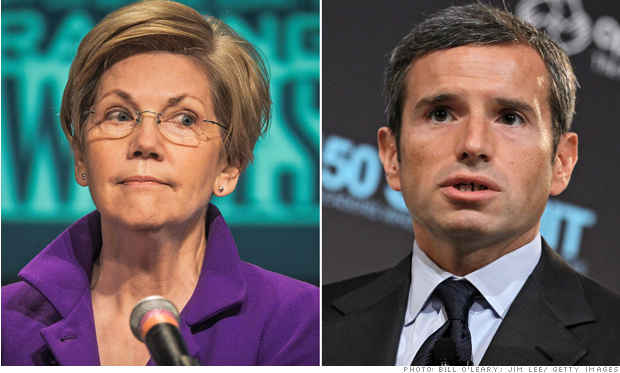
\includegraphics[height=2.6in,width=4in]{WarrenWeiss.png}

Elizabeth Warren and Antonio Weiss
\end{center}

\end{frame}

\begin{frame}

\frametitle{What Do We Know About Appointments?}
\begin{itemize}\addtolength{\itemsep}{0.25\baselineskip}
\item Scholars have been particularly concerned with politicization of the bureaucracy (e.g. Hart 1995; Heclo 1975; Lewis 2005, 2008). 
\item Tradeoff between political loyalists and experts (e.g. Hollibaugh forthcoming; Moe 1985; Parsneau 2013).
\begin{itemize}
\item While experts cannot be trusted to advance the president's political interests (Moe 1985)...
\item ...loyalists lack the skill to execute policy well or efficiently (e.g.Lewis 2005; Gilmour and Lewis 2006; Heclo 1975, 1977).
\end{itemize}
\item Presidents may decide based on patronage considerations (e.g. Hollibaugh et al. forthcoming; Patterson 2008; Tolchin and Tolchin 2010).
\item Low-level appointees largely slip under the radar of media and congressional oversight (Lewis and Waterman 2013).  
\end{itemize}
\end{frame}


\begin{frame}
\frametitle{What Don't We Know About Appointments?}

\begin{itemize}\addtolength{\itemsep}{1.25\baselineskip}
\item Presidents have many options in their toolkits for advancing policy (e.g. Rudalevige 2002). Staffing is one of those tools.
\item While influence is largely studied, attention is not.
\begin{itemize}
\item We do not know how presidents allocate finite administrative resources.
\end{itemize}
\item Agenda Setting and issue agenda literature largely focused on how the
media or public opinion shapes the agenda the president pursues with Congress (e.g. Cohen
1995; Edwards and Wood 1999; Hill 1998).

\end{itemize}
\end{frame}

\begin{frame}

\frametitle{Why Would Attention Vary Across Agencies}
\begin{itemize}\addtolength{\itemsep}{0.5\baselineskip}
\item Agencies may differ in their willingness to follow the president's directives based on the ideological leaning of the agency (Aberbach and Rockman 1976, 1995, 2000; Bertelli and Grose 2009; Clinton and Lewis 2008; Clinton et al. 2012; Hollibaugh et al. forthcoming)
\item It is not obvious which way this relationship would go.
\begin{itemize}
\item Presidents could support agencies which are ideologically similar.
\item But an argument could just as easily be made that presidents support ideologically dissimilar agencies. 
\end{itemize}
\item No clear theory for how bureaucratic agencies are operated internally.
\item Appointments present an opportunity cost. An appointment in one area is not available for an appointment elsewhere. 
\end{itemize}
\end{frame}

\begin{frame}
\frametitle{Excepted Service and Attention}

\begin{columns}[T] % align columns
\begin{column}{.48\textwidth}

\begin{itemize}\addtolength{\itemsep}{1.5\baselineskip}
\item There are many different types of Excepted Service Appointments.
\item Excepted Service Appointments are flexible.
\item Excepted Service Appointments do not undergo advice and consent.
\end{itemize}
\end{column}%
\hfill%
\begin{column}{.48\textwidth}

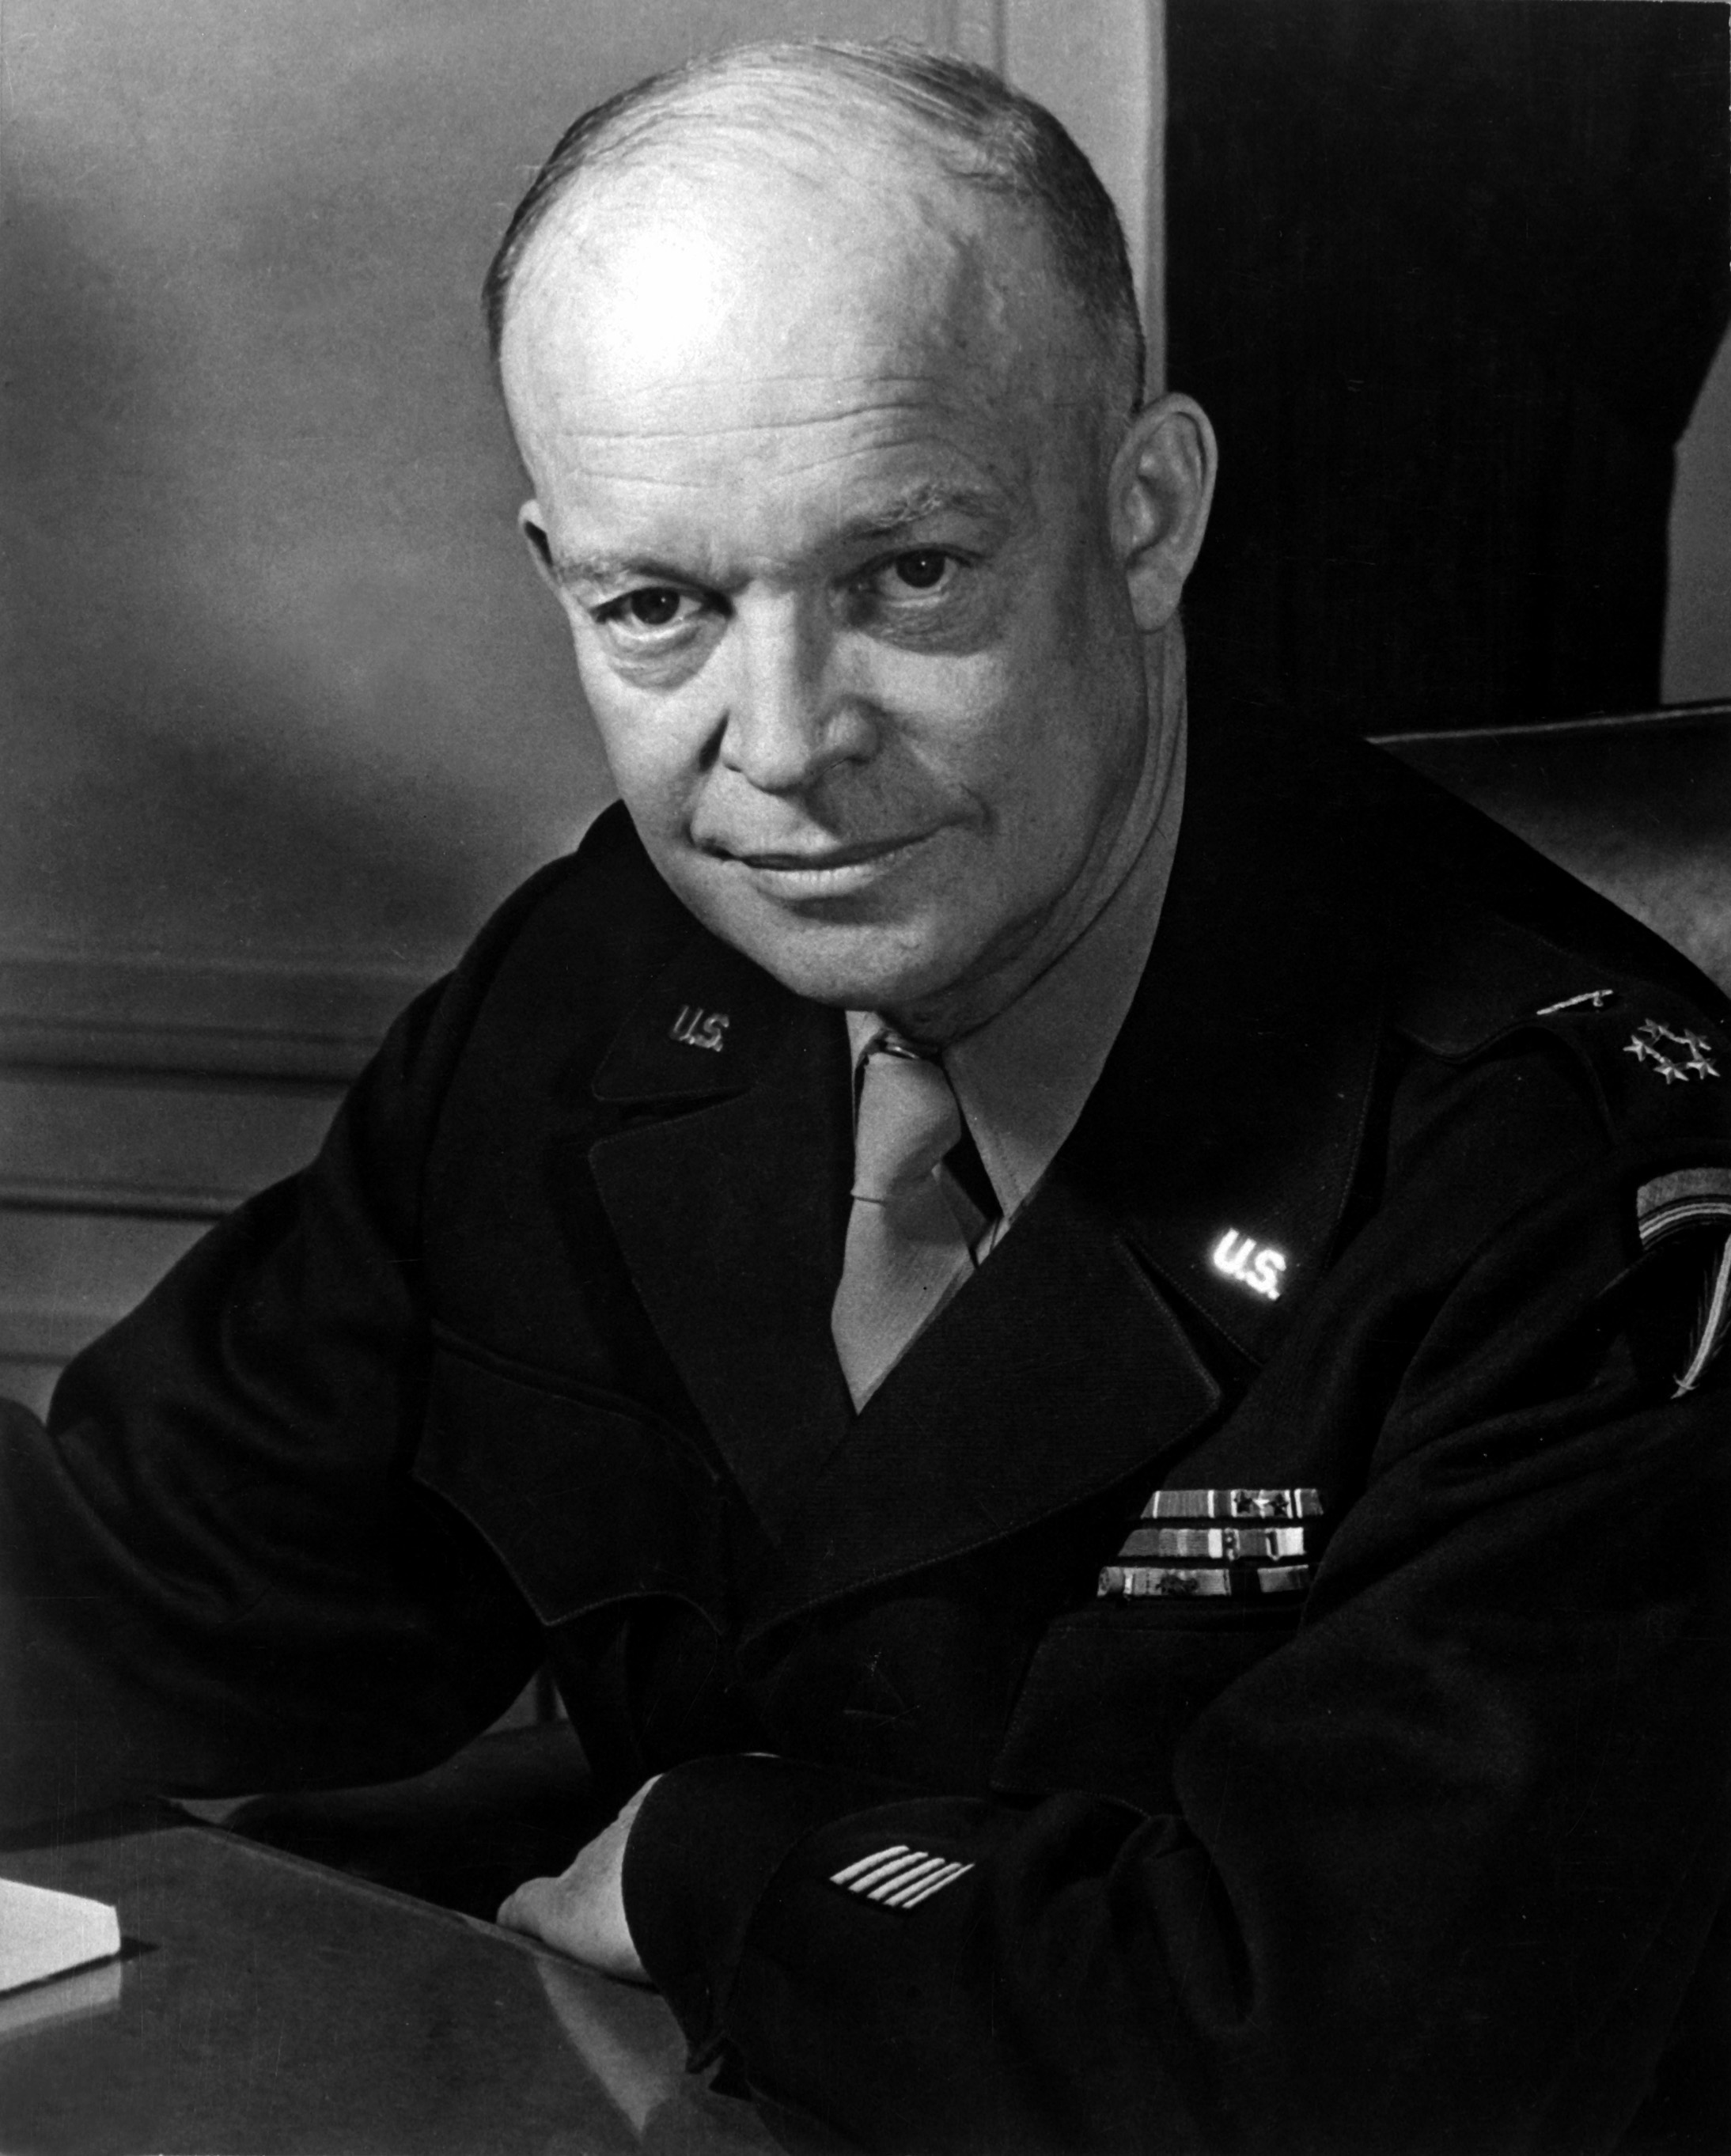
\includegraphics[height=2.5in,width=2in]{eisenhower.jpg}
\end{column}%
\end{columns}
\end{frame}

\begin{frame}
\begin{center}
\includegraphics[height=3.7in,width=4.5in]{RPlot.pdf}
\end{center}
\end{frame}

\begin{frame}
\frametitle{Expectations}

\begin{itemize}\addtolength{\itemsep}{1.5\baselineskip}
\item We expect that president will use these flexible appointments especially in urgent situations. 
\item We expect that agencies tasked with communicating the president's message to Congress or the public to be staffed using Excepted Service.
\item We expect that agency ideology will be connected with staffing by Excepted Service.
\item We expect changes in attention between presidents to reflect their relative agendas. 
\end{itemize}
\end{frame}

\begin{frame}
\frametitle{Data}
\begin{itemize} \addtolength{\itemsep}{1.5\baselineskip}
\item OPM produces an online "statistical datamart," which includes information about most federal employees and most agencies from 1998-2013. 
\item Few studies utilize this data.
\item 692 agencies exist over the period with varying levels of agency aggregation.
\item Within the agency, we can determine total employment broken down by appointment type. 
\end{itemize}
\end{frame}

\begin{frame}
\frametitle{Urgency}
\begin{figure}[htb]
\begin{center}
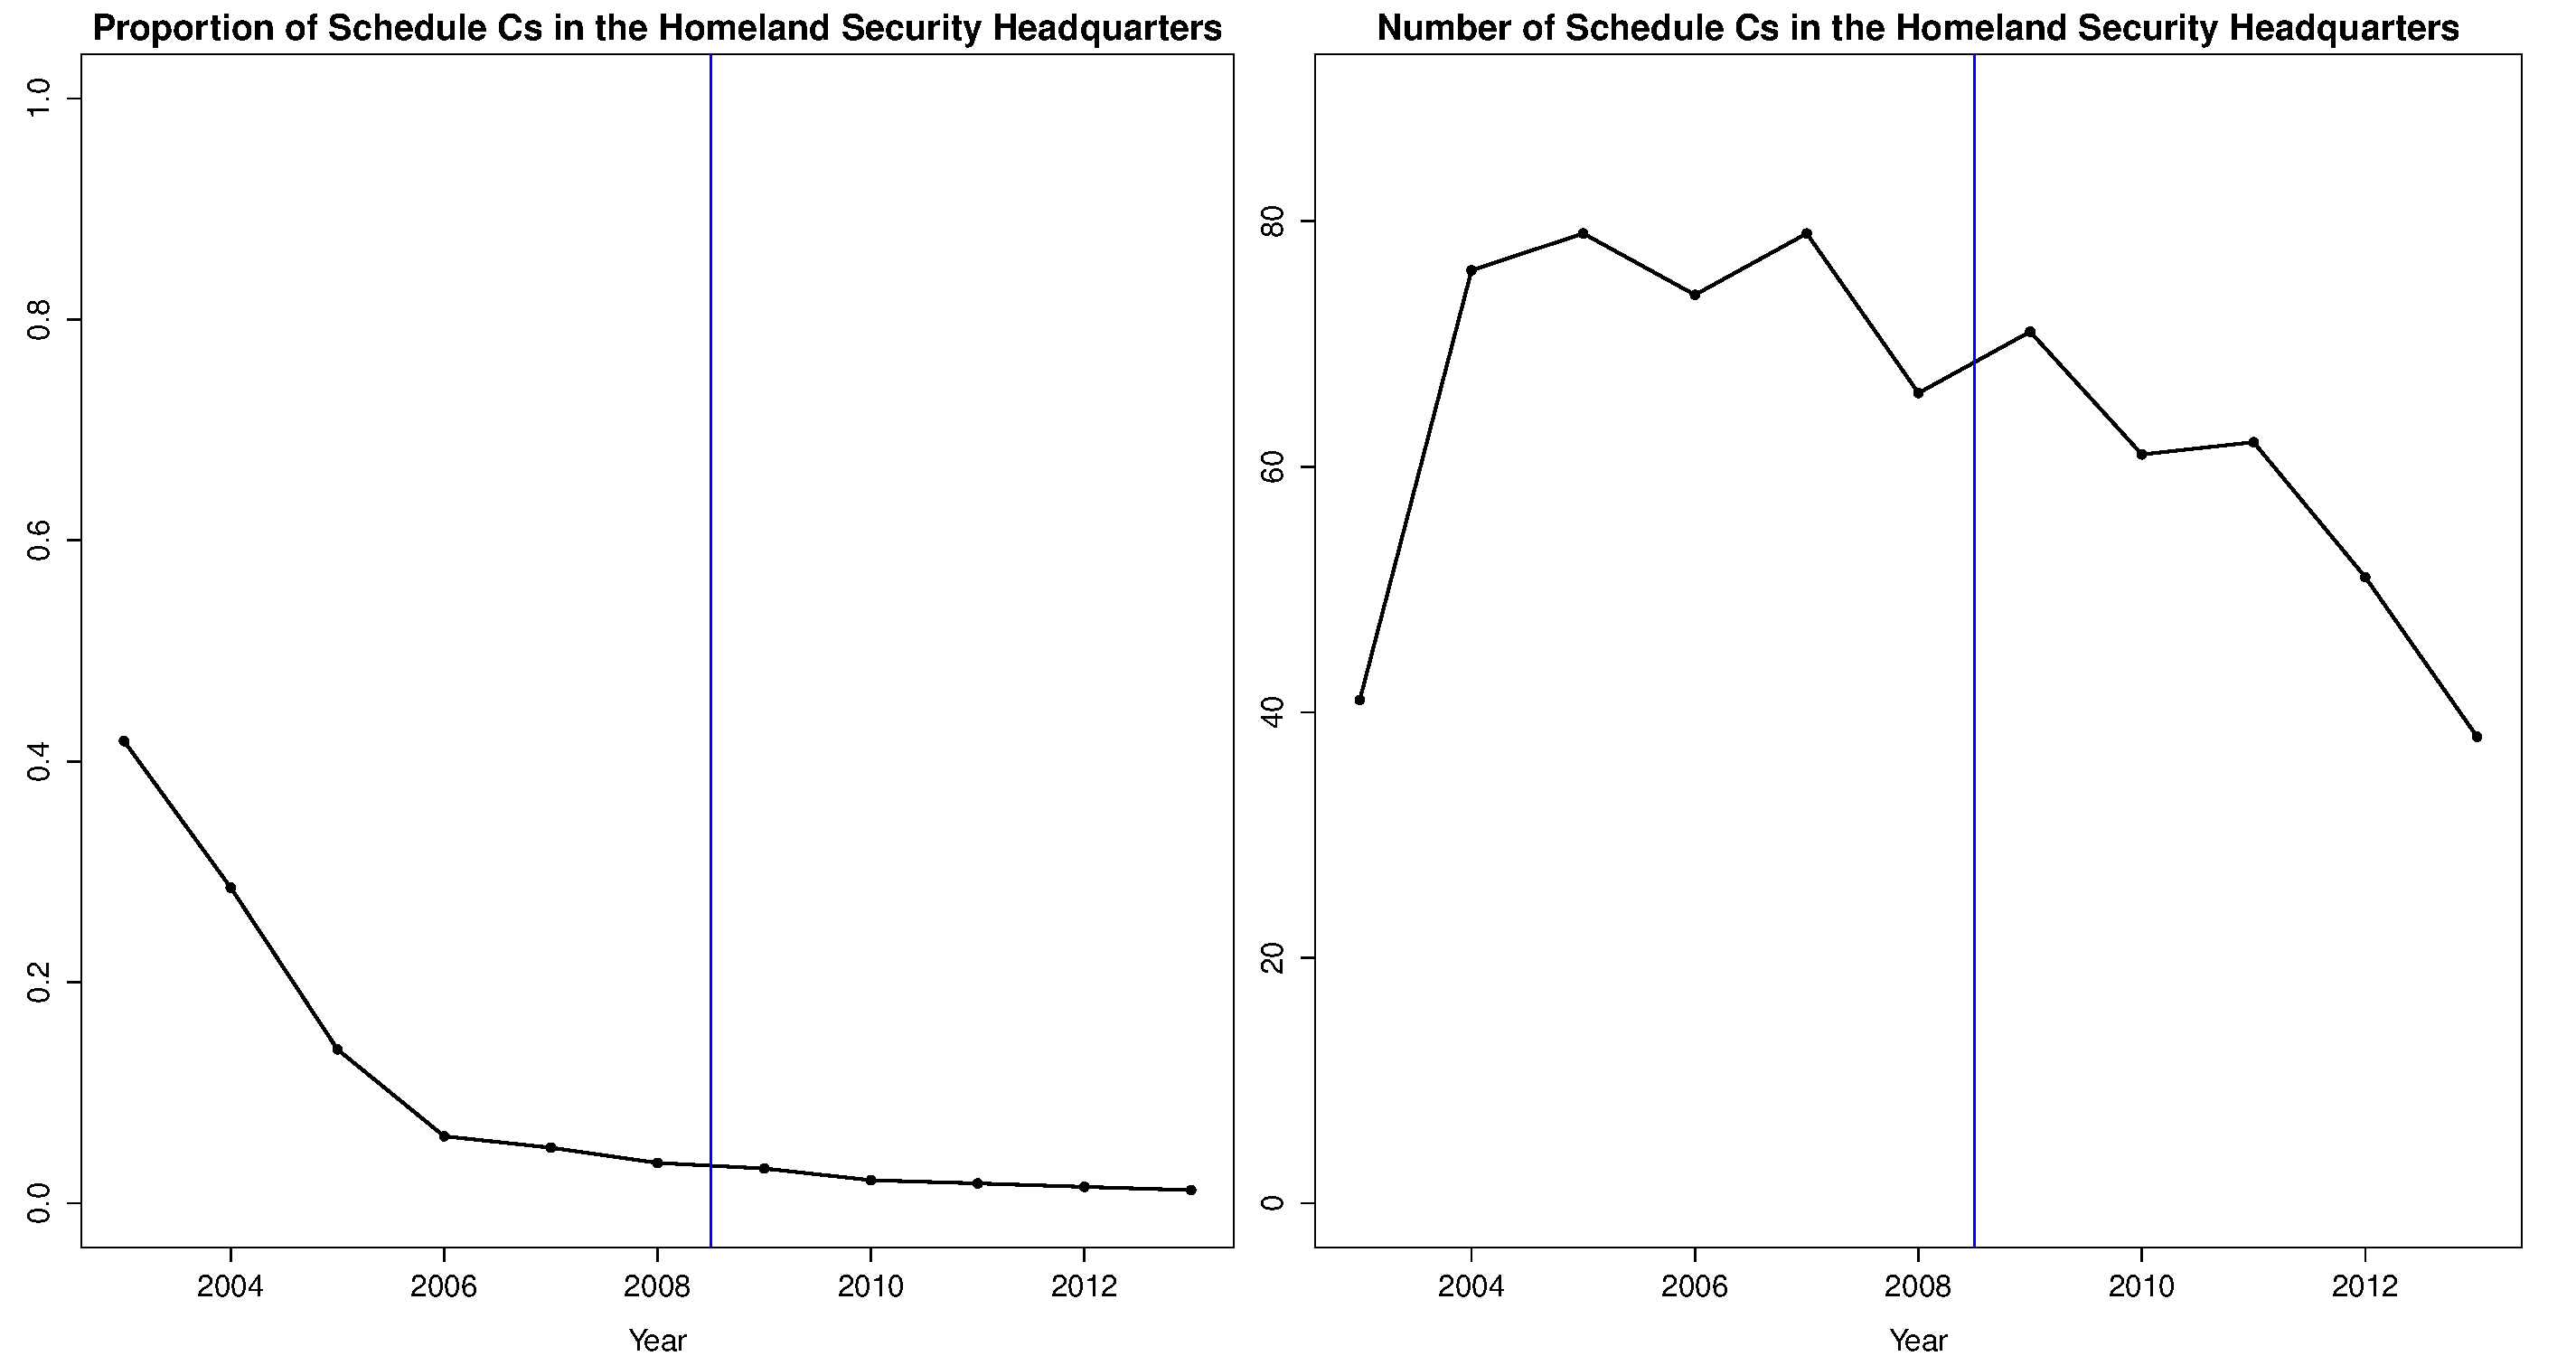
\includegraphics[height=2.75in,width=4.9in]{DHSProportionRawNumber.pdf}
\end{center}
\end{figure}
\end{frame}

\begin{frame}
\frametitle{Liaison Agencies}
\begin{center}
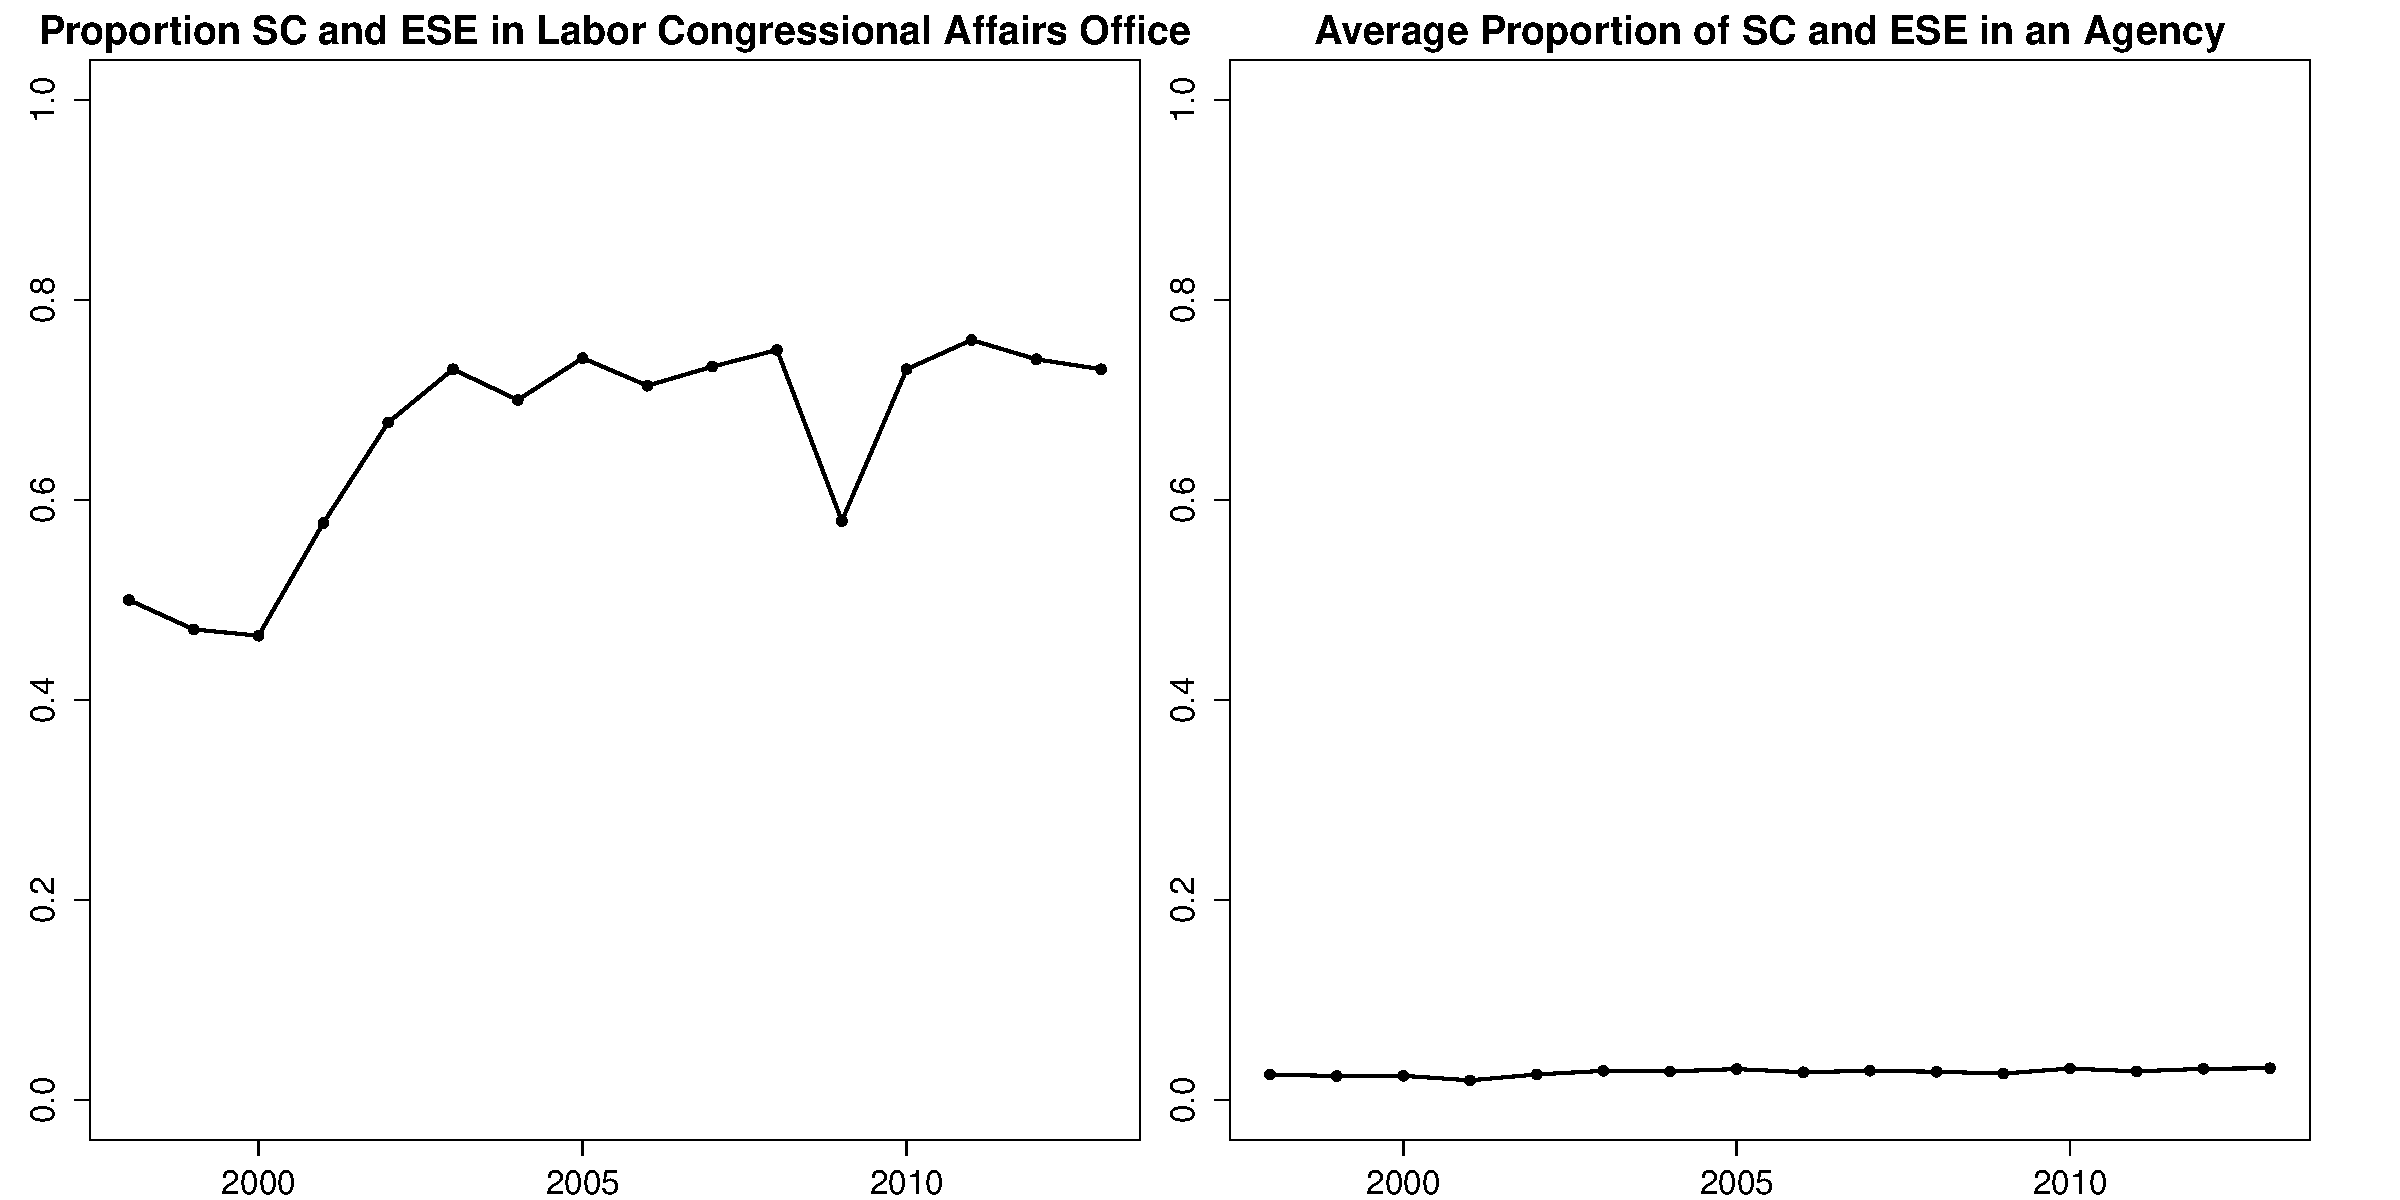
\includegraphics[height=2.5in,width=4.8in]{LaborCongressionalAffairs.pdf}
\end{center}
\end{frame}

\begin{frame}
\frametitle{Attention and Ideology}

\begin{itemize}\addtolength{\itemsep}{1.5\baselineskip}
\item The result is meant to serve as a validation of using Schedule C and ESE appointments to study attention. 
\item Ideology is measured as the absolute distance between the agency ideal point and the president's ideal point.
\item Negative Binomial Regression Model.
\begin{itemize}\addtolength{\itemsep}{1\baselineskip}
\item Outcome Variable: Counts of Schedule C and ESE appointments in each agency 1998-2013.
\item Model includes ideology measure, presidential dummies, and agency fixed effects.
\end{itemize}
\end{itemize}
\end{frame}

\begin{frame}[fragile]
\frametitle{Ideology}
\begin{columns}[T] % align columns
\begin{column}{.48\textwidth}
\begin{center}
\begin{table}[!htb] \centering 
\tiny 
  \label{} 
\begin{tabular}{@{\extracolsep{1pt}}lcccccc} 
\\[-1.8ex]\hline 
\hline \\[-1.8ex] 
 & \multicolumn{2}{c}{\textit{Dependent variable:}} \\ 
\cline{2-3} 
\\[-1.8ex] & \multicolumn{2}{c}{SC and ESE Apts} \\ 
\hline \\[-1.8ex] 
 Ideology & 0.218 & 0.058 \\ 
  & (0.06) & (0.023) \\ 
  & &\\ 
 Bush & 0.048 & 0.007 \\ 
  & (0.110) & (0.023) \\ 
  & &\\ 
 Obama & 0.018 & $-$0.018 \\ 
  & (0.118) & (0.025) \\ 
  & &\\ 
 Constant & 3.08& $-$0.011 \\ 
  & (0.108)& (0.506) \\ 
  & &\\ 
\hline \\[-1.8ex] 
Agency Fixed Effects & No & Yes \\
Observations & 1,213 & 1,213\\ 
Log Likelihood & $-$5,047.143 & $-$3,140.066 \\ 
$\theta$ & 0.513(0.019)& 51.100 (6.226) \\ 
Akaike Inf. Crit. & 10,102.290 & 6,442.132& \\ 
\hline 
\hline \\[-1.8ex] 
\end{tabular} 
\end{table} 
\end{center}
\end{column}
\begin{column}{.48\textwidth}
\begin{center}
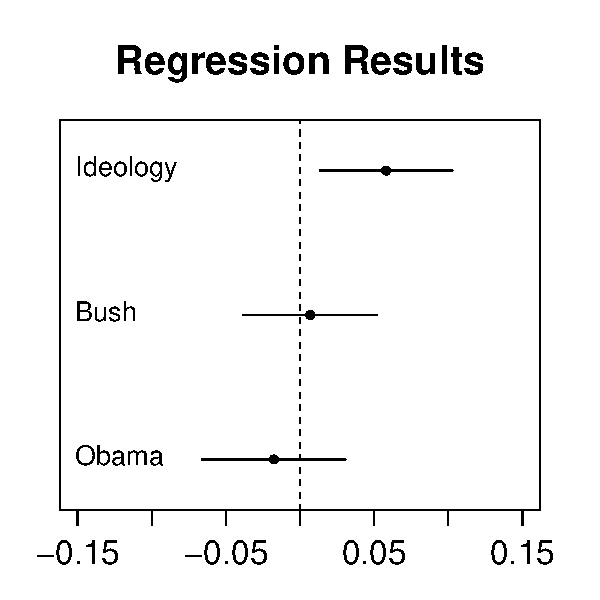
\includegraphics[height=2.25in,width=2.25in]{RegressionResults.pdf}
\end{center}
\end{column}
\end{columns}
\end{frame}

\begin{frame}[fragile]
\frametitle{Share of Attention}

\begin{itemize}\addtolength{\itemsep}{1\baselineskip}
\item Looking at which agencies receive the largest share of the total Schedule C and ESE appointments is another way to look at attention. 
\item Of the total Schedule C and ESE appointments, which agencies are getting more or less?
\item The changes in the share of attention should be suggestive of differences in the president's agenda at different time periods.
\item This analysis seeks to capture policy dimensions, not the ideological dimension.

\end{itemize}
\end{frame}

\begin{frame}[fragile]
\frametitle{Appointments and Presidential Priorities}
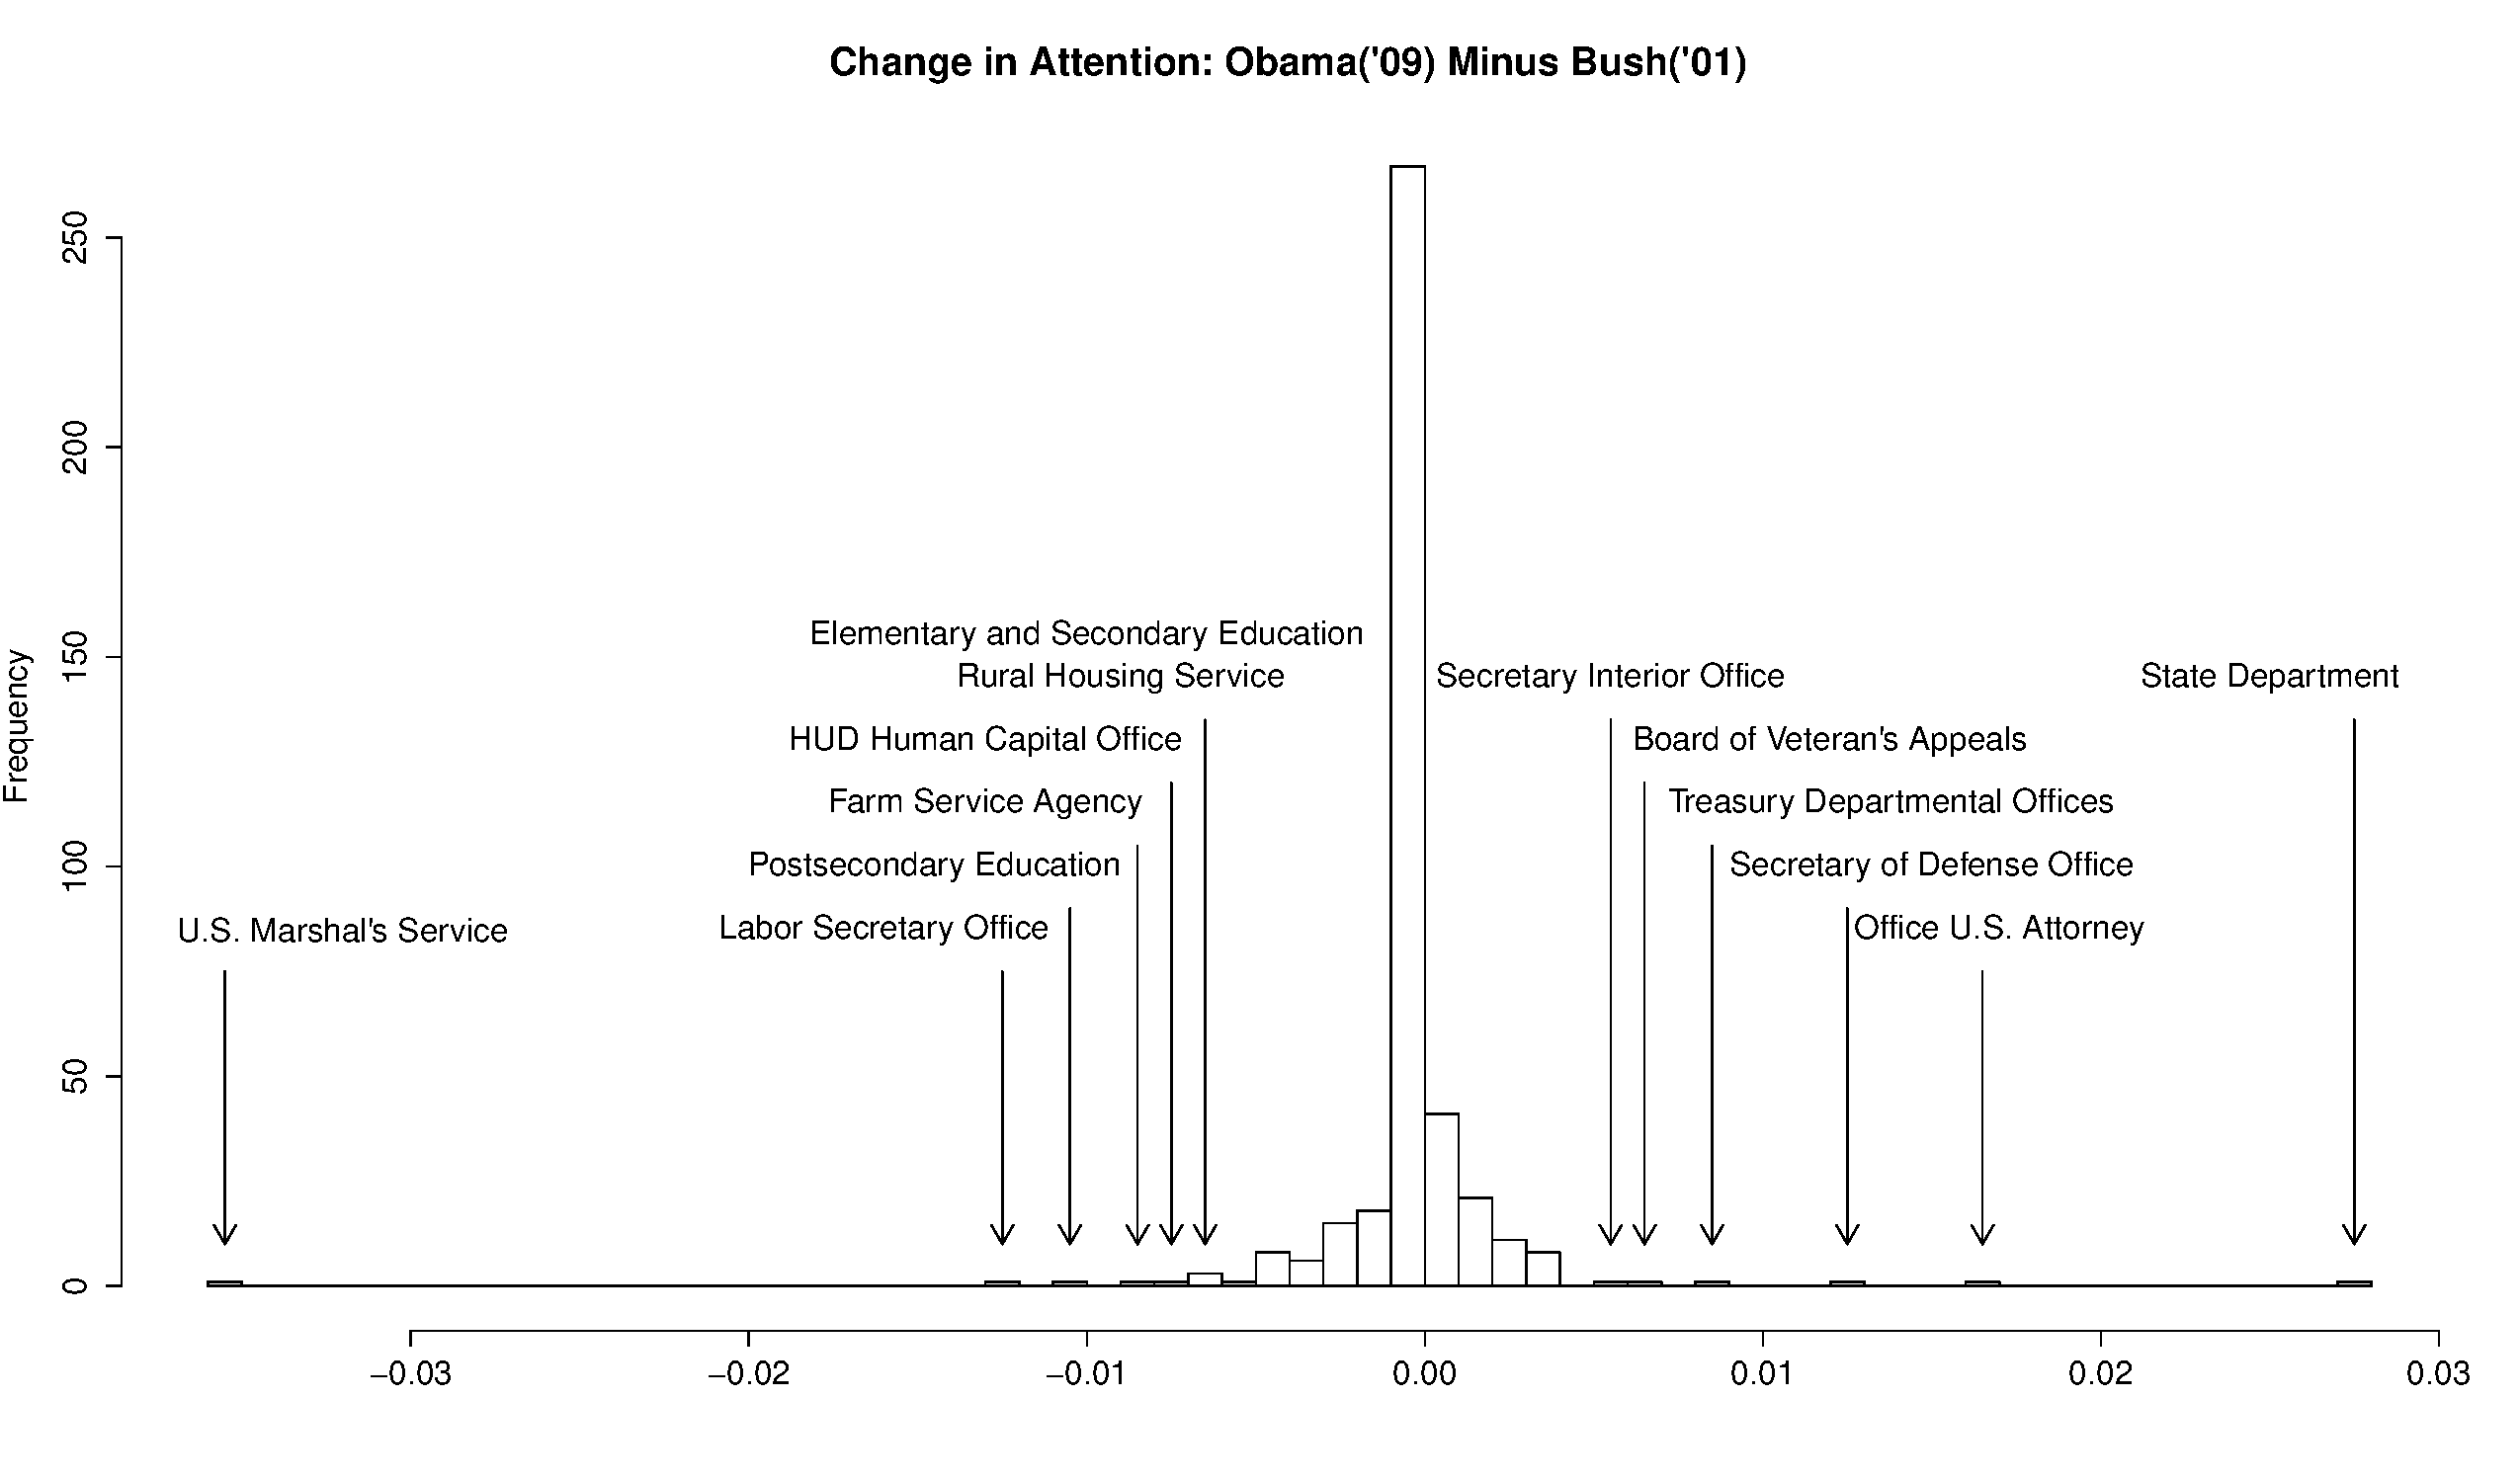
\includegraphics[height=3.2in,width=4.9in]{AttentionChange01to09.pdf}
\end{frame}

\begin{frame}[fragile]
\frametitle{Appointments and Presidential Priorities}
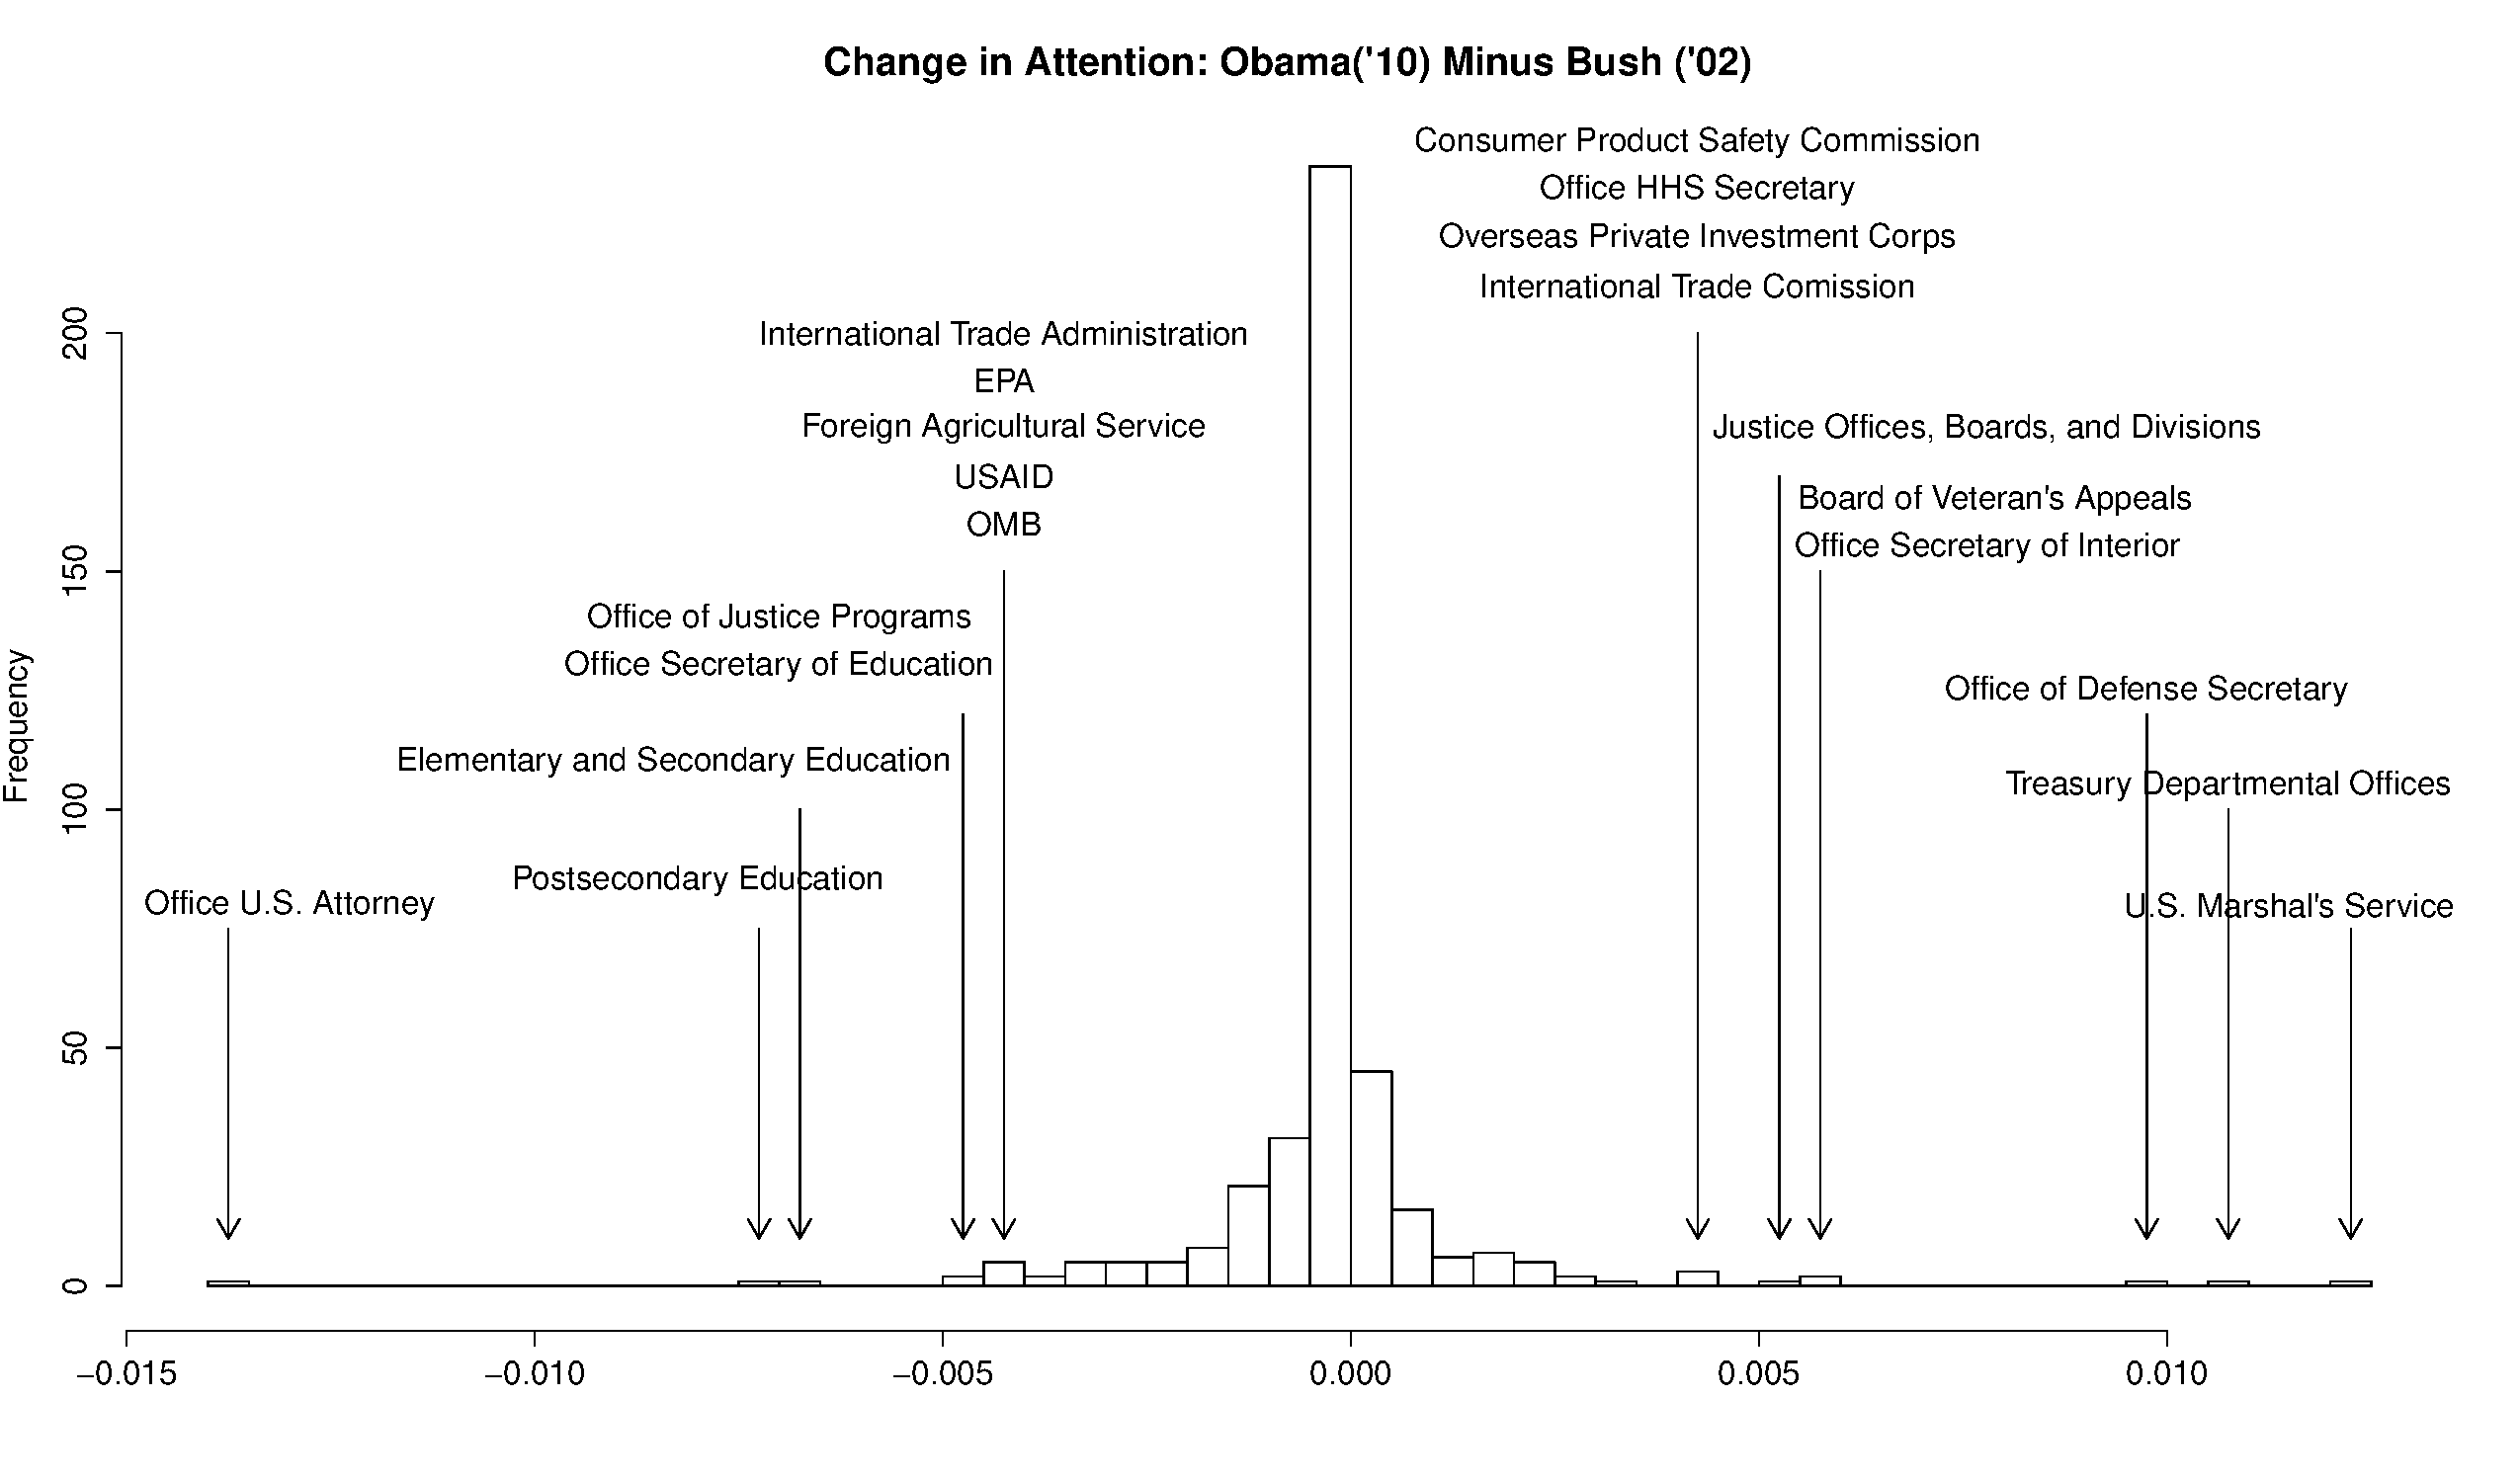
\includegraphics[height=3.2in,width=4.9in]{AttentionChange02to10.pdf}
\end{frame}

\begin{frame}[fragile]

\frametitle{Conclusion}
\begin{itemize}\addtolength{\itemsep}{0.5\baselineskip}
\item Attention is important but understudied
\item We know little about how presidents apportion their more flexible personnel.
\item Schedule C and Excepted Service Executive Appointments appear to be good for measuring attention.
\begin{itemize}
\item As we would expect, there are high proportions of these appointments in a new agency, which then declines over time.
\item Also as expected, liaison agencies have consistently high proportions of these appointments for all presidents.
\item Ideology is correlated with counts of these appointments. The negative relationship might be suggestive for future theory-building.
\item Changes in shares of attention do appear suggestive of elements of the Bush and Obama agendas. 
\end{itemize}

\end{itemize}
\end{frame}

\begin{frame}
\frametitle{Bush and Obama Unified and Divided}

\begin{table}[!htbp] \centering 
\tiny
\begin{tabular}{@{\extracolsep{5pt}} lllllll} 
\\[-1.8ex]\hline 
& More Attention in 2006 &&& More Attention in 2007 & \\
\hline \\[-1.8ex] 
DJ09 & Office U.S. Attorney & -0.00641          & DN00 & Department of Energy &  0.00414 \\ 
DJ01 & Just. Ofs, Boards, and Divs. & -0.00465& DD01 & Ofc. Secretary Defense& 0.00374 \\ 
HSDA & Nuclear Detection Office& -0.00434     & NF00 & Natl Science Found.& 0.00371 \\ 
DD34 & Defense Commissary Agency & -0.00257   & TC00 & U.S. Intl Trade Comm. & 0.00286 \\ 
DJ07 & Ofc. of Justice Programs & -0.00219    & TR91 & Treas. Departmental Ofcs. & 0.00261 \\ 
CM54 & NOAA &  -0.00217                       & AH03 & Inst. Museum and Library Serv.& 0.00244 \\ 
NV18 & Naval Medical Command & -0.00173       & SB00 & Small Business Admin. & 0.00234 \\ 
IB00 & Broadcasting Board of Govs. & -0.00172 & VAAD & Board Veteran's Appeals& 0.0021 \\ 
CM51 & Office Sec. Commerce &  -0.00153       & AH01 & Natl Endowment Arts & 0.00202 \\ 
EP00 & EPA & -0.00153                         & AG07 & Rural Housing & 0.00186 \\ 
\hline \\[-1.8ex] 
\end{tabular} 
\end{table}

\begin{table}[!htbp] \centering 
\tiny
\begin{tabular}{@{\extracolsep{5pt}} llllll} 
\\[-1.8ex]\hline 
& More Attention in 2010 &&& More Attention in 2011 & \\
\hline \\[-1.8ex] 
DN00 & Department of Energy       & -0.00752 & DJ08 & U.S. Marshal's Service & 0.00907 \\ 
TR91 & Treasury Departmental Offices  & -0.00619 & AF13 & USAF HQ and Support &  0.00478 \\ 
EDEA & Secretary of Education          & -0.00527 & EDEE & Undersec. of Education &  0.0039 \\ 
AF0N & HQ USAF                    & -0.00349 & DJ09 & Office U.S. Attorney     & 0.00381 \\ 
CM51 & Secretary Commerce         & -0.00267 & VAAD & Board Veteran's Appeals & 0.00346 \\ 
IN01 & Secretary Interior         & -0.00267 & AM00      & USAID &  0.0026 \\ 
HSDA & Nuclear Detection Office     & -0.00262 & SB00 & Small Business Admin. & 0.00256 \\ 
DJ01 & Justice Offices, Boards, and Divs & -0.00228 & AG01 & Office Secretary Agriculture & 0.00213 \\ 
DD60 & DOD Tricare Management     & -0.00218 & SZ00 & Social Security Admin. & 0.00174 \\ 
ST00 & State Department           & -0.00192 & FW00 & Office of Special Counsel& 0.00174 \\ 
\hline \\[-1.8ex] 
\end{tabular} 
\end{table}
\end{frame}

\begin{frame}
\frametitle{Zero Inflated Negative Binomial}
\begin{table}[!htbp] \centering 
\begin{tabular}{@{\extracolsep{5pt}}lc} 
\\[-1.8ex]\hline 
\hline \\[-1.8ex] 
 & \multicolumn{1}{c}{\textit{Dependent variable:}} \\ 
\cline{2-2} 
\\[-1.8ex] & AllCount \\ 
\hline \\[-1.8ex] 
 abs(Ideo) & 0.059$^{***}$ \\ 
  & (0.023) \\ 
  & \\ 
 Bush & 0.008 \\ 
  & (0.023) \\ 
  & \\ 
 Obama & $-$0.014 \\ 
  & (0.025) \\ 
  & \\ 
 Constant & $-$0.015 \\ 
  & (0.505) \\ 
  & \\ 
\hline \\[-1.8ex] 
Observations & 1,213 \\ 
Log Likelihood & $-$3,135.422 \\ 
\hline 
\hline \\[-1.8ex] 
\textit{Note:}  & \multicolumn{1}{r}{$^{*}$p$<$0.1; $^{**}$p$<$0.05; $^{***}$p$<$0.01} \\ 
\end{tabular} 
\end{table} 
\end{frame}


\end{document}









